%% fig_markov_chain.tex  —  Agent Markov chain transition diagram.
%% Compile: pdflatex fig_markov_chain.tex
%% Uses the running 3-state example from definitions.tex (m=3).
%%
\documentclass[tikz, border=8pt]{standalone}
\usepackage{tikz}
\usetikzlibrary{arrows.meta, positioning, shapes.geometric, fit, backgrounds}

%% ── colour palette ──────────────────────────────────────────────────────────
\definecolor{mcblue}{RGB}{30,90,180}          % transient state fill
\definecolor{mcgreen}{RGB}{34,139,80}         % success (⊕) fill
\definecolor{mcred}{RGB}{192,40,40}           % failure (⊖) fill
\definecolor{mclightblue}{RGB}{210,228,255}   % transient background
\definecolor{mcarrow}{RGB}{60,60,60}          % arrow colour

\begin{document}
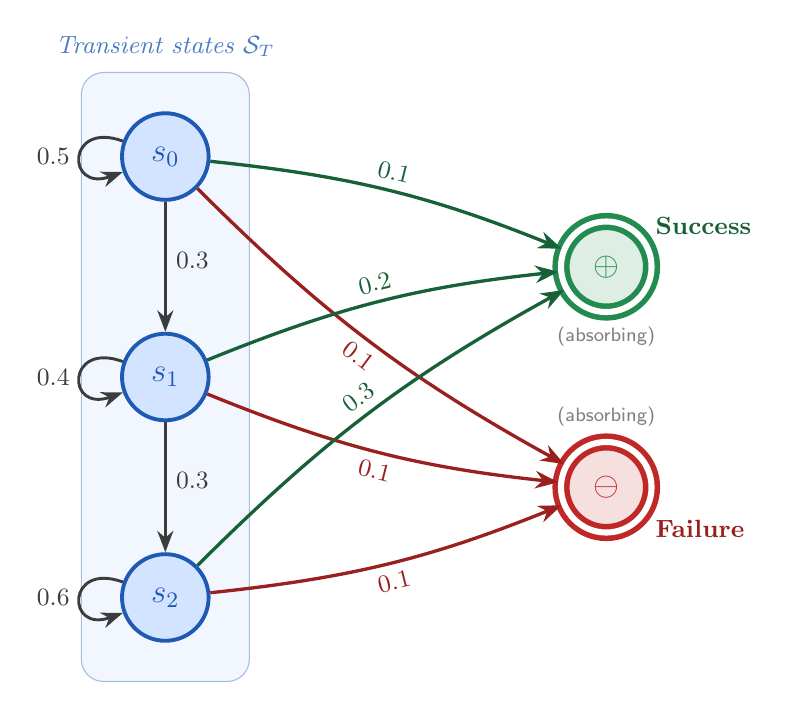
\begin{tikzpicture}[
    >=Stealth,
    %% ── node styles ──────────────────────────────────────────────────────────
    transient/.style={
        circle, draw=mcblue, fill=mclightblue,
        line width=1.4pt, minimum size=1.1cm,
        font=\large\bfseries, text=mcblue
    },
    absorbing/.style={
        circle, draw=#1, fill=#1, fill opacity=0.15, text opacity=1,
        line width=2pt, minimum size=1.15cm,
        font=\large\bfseries, text=#1,
        double, double distance=2.2pt, double=white
    },
    %% ── edge styles ──────────────────────────────────────────────────────────
    trans/.style={
        ->, draw=mcarrow, line width=1.05pt,
        font=\small\sffamily, color=mcarrow
    },
    tosucc/.style={
        ->, draw=mcgreen!80!black, line width=1.2pt,
        font=\small\sffamily, color=mcgreen!70!black
    },
    tofail/.style={
        ->, draw=mcred!80!black, line width=1.2pt,
        font=\small\sffamily, color=mcred!80!black
    },
]

%% ── Transient states (left column: s0 top, s1 middle, s2 bottom) ─────────────
\node[transient] (s0) at (0, 2.8)  {$s_0$};
\node[transient] (s1) at (0, 0)    {$s_1$};
\node[transient] (s2) at (0,-2.8)  {$s_2$};

%% ── Absorbing states (right column) ─────────────────────────────────────────
\node[absorbing=mcgreen] (succ) at (5.6, 1.4)  {$\oplus$};
\node[absorbing=mcred]   (fail) at (5.6,-1.4)  {$\ominus$};

%% ─────────────────────────────────────────────────────────────────────────────
%% Q-block: transitions among transient states
%% ─────────────────────────────────────────────────────────────────────────────

%% s0 → s0 self-loop
\draw[trans] (s0) edge[loop left, looseness=5,
              out=160, in=200] node[left] {$0.5$} (s0);

%% s0 → s1
\draw[trans] (s0) -- node[right, pos=0.45] {$0.3$} (s1);

%% s1 → s1 self-loop
\draw[trans] (s1) edge[loop left, looseness=5,
              out=160, in=200] node[left] {$0.4$} (s1);

%% s1 → s2
\draw[trans] (s1) -- node[right, pos=0.45] {$0.3$} (s2);

%% s2 → s2 self-loop
\draw[trans] (s2) edge[loop left, looseness=5,
              out=160, in=200] node[left] {$0.6$} (s2);

%% ─────────────────────────────────────────────────────────────────────────────
%% R-block: absorption edges
%% ─────────────────────────────────────────────────────────────────────────────

%% s0 → ⊕  (0.1)   s0 → ⊖  (0.1)
\draw[tosucc] (s0) to[bend left=8]  node[above, sloped] {$0.1$} (succ);
\draw[tofail] (s0) to[bend right=8] node[below, sloped] {$0.1$} (fail);

%% s1 → ⊕  (0.2)   s1 → ⊖  (0.1)
\draw[tosucc] (s1) to[bend left=8]  node[above, sloped] {$0.2$} (succ);
\draw[tofail] (s1) to[bend right=8] node[below, sloped] {$0.1$} (fail);

%% s2 → ⊕  (0.3)   s2 → ⊖  (0.1)
\draw[tosucc] (s2) to[bend left=8]  node[above, sloped] {$0.3$} (succ);
\draw[tofail] (s2) to[bend right=8] node[below, sloped] {$0.1$} (fail);

%% ─────────────────────────────────────────────────────────────────────────────
%% Legend / region labels
%% ─────────────────────────────────────────────────────────────────────────────
\begin{scope}[on background layer]
  %% Transient region shading
  \node[draw=mcblue!40, fill=mclightblue!30, rounded corners=8pt,
        fit=(s0)(s1)(s2), inner sep=14pt] (transbox) {};
\end{scope}

\node[text=mcblue!80, font=\small\itshape, above=2pt of transbox]
    {Transient states $\mathcal{S}_T$};

\node[text=mcgreen!70!black, font=\small\bfseries, above right=-4pt and 2pt of succ]
    {Success};
\node[text=mcred!80!black, font=\small\bfseries, below right=-4pt and 2pt of fail]
    {Failure};

%% Block labels beneath absorbing nodes
\node[font=\scriptsize\sffamily, text=gray, below=1pt of succ] {(absorbing)};
\node[font=\scriptsize\sffamily, text=gray, above=1pt of fail] {(absorbing)};

\end{tikzpicture}
\end{document}
